\chapter{Análise e discussão dos resultados}

\section{Simulador}

O uso do simulador foi importantíssimo para o desenvolvimento desse trabalho. Ele possibilitou iniciar o desenvolvimento sem uma placa física. Utilizando-o montou-se um circuito exemplo utilizando o microcontrolador escolhido e, de forma iterativa, era possível evoluir tanto o circuito quanto o software, por exemplo: montou-se o circuito com o LCD e implementou-se o módulo de controle do mesmo, adicionou-se os componentes de menu e a análise de botões, e outros passos. Vendo esses passos é possível perceber que o desenvolvimento foi feito por funcionalidade isoladas de forma que fosse possível testar cada "parte" do software e assim minimizar os problemas do \emph{software} como um todo e assim sempre ter um versão estável, mesmo que mínima.

Além de todas essas facilidades, a gama de testes e depuração é maior em um simulador do que no \emph{hardware}, como: o simulador indica más práticas existentes, permite simular o uso da bomba por dias em questão de minutos, basta configurar o tempo de execução, e outros. Graças aos exemplos citados anteriormente foi possível encontrar diversos problemas que só seriam descobertos quando estivesse testando diretamente no \emph{hardware} e mesmo assim surgiria a dúvida: É o \emph{hardware} ou o \emph{software}.

O circuito elétrico utilizado para os testes foi desenvolvido com base na placa Microgenios, representada pela Figura \ref{fig:microgenios}. Todos os componentes utilizados assim como as ligações entre eles são fiéis à placa de referência, salvo às ligações do motor que não faz parte do conjunto de referência. Portanto uma migração para a placa de Microgenios teria o funcionamento dos botões existentes e \emph{display} de LCD de acordo com o esperado.

E, além disso, como os testes e validações do \emph{hardware} feito através simulador são extremamente válidas e consistentes e o desenvolvimento foi baseado em uma placa consolidada, uma integração com uma placa diferente da utilizada como referência será muito mais simples. Isso deve-se ao fato através do simulador diminui-se os riscos e problemas no período de integração, onde são encontrados as maiores e inesperadas dificuldades do desenvolvimento.
 
 \newpage
 
 \begin{figure}[htp]
 	\centering
 	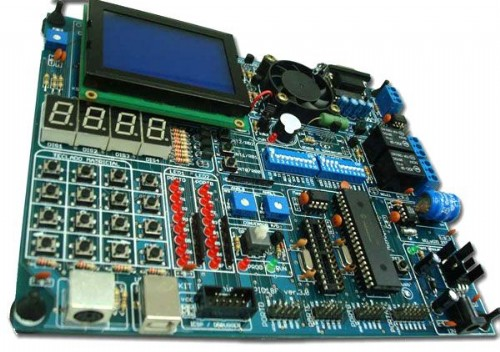
\includegraphics[scale=1]{images/pic_microgenio.png}
 	\caption{Placa Microgenios PIC18F4452}	
 	\label{fig:microgenios}
 	\cite{galvao2013requirements}
 \end{figure}

\section{Arquitetura modularizada}

A forma com que foi organizado o código é a grande vantagem desse trabalho. O desacoplamento foi o foco principal durante todo o desenvolvimento isso para facilitar mudanças no próprio \emph{software} ou mudança do \emph{hardware}

OOC foi o conceito utilizado para que fosse possível fazer testes, mocks no sistema, pelo fato de simular programação orientação à objetos. Devido a forma com que foi implementado, foi possível realizar testes utilizando um PC. O ambiente utilizado: Ubuntu 13.10, compilador gcc, Framework C++ Qt e IDE QtCreator. Como o conceito de OOC é baseado em ponteiros de função o mock das funções foi feito apenas apontando para uma função que foi criada de acordo com a situação de teste desejada. Quanto o acesso aos periféricos, todos os acionamentos e comunicações foram redirecionadas para um arquivo log de acompanhamento. A seguir será descrito as vantagens principais de cada módulo devido a forma de implementação.

O módulo Config é o mais simples de todos, Sua principal vantagem é o fato de centralizar todas as informações de configuração, fazendo com que o sistema fique mais claro. Além disso, criar casos de testes torna-se simples, pois mudando qualquer uma de suas informações já se reflete no sistema com um todo. É importante lembrar também que ele não carrega nenhuma dependência do compilador ou do hardware, foi implementado em ANSI-C, o que permite que seja utilizado por qualquer compilador e \emph{hardware}.

Os demais módulos foram criados para seguir a ideia de isolação do módulo config. Para isso o que foi feito é deixar as interfaces e funções comuns independente de \emph{hardware} e compilador utilizando apenas ANSI-C. Dessa forma, caso precise de alguma mudança mais drástica relacionada aos dois itens citados o impacto seja mínimo, precisando fazer apenas um de-para das funcionalidades específicas. 

Tendo dito as vantagens com relação à mudanças \emph{hardware} e compilador é importante lembrar que a expansibilidade e manutenibilidade do software ficou incrivelmente simples. A ideia foi deixar o "motor" ou "coração" da bomba ter conhecimento apenas das "interface" do sistemas. Dessa forma os detalhes de funcionamento, requisitos de segurança, configurações específicas de hardware para controle dos periféricos e outros, podem ser modificadas sem impactar o funcionamento básico da bomba de infusão. O mais importante é que essas alterações são parametrizável,se localizam no módulo config, e o software sabe quais objetos utilizar e de onde recuperá-los, em algum \emph{Factory} na maioria dos casos. Devido a isso tudo é possível manter mais de um produto em um único código e mudanças importantes no \emph{core} do sistema não precisa ser replicadas e correr risco de conflito entre projetos. Graças ao uso do OOC para criar algo novo basta implementar as funções da interface do módulo em questão e adicionar ao \emph{factory}, caso exista. Segue uma breve explicação do que pode ser feito em cada módulo.

O módulo InsulinPump, responsável por abstrair particularidades de funcionalidades e segurança do bomba para o resto do ambiente permite que se crie vários tipos de bomba. Essa criação leva em conta mudanças nos dois itens citados, por exemplo, bomba europeia, americana, brasileira, que podem ter requisitos de segurança distintos.

O módulo LCD, responsável por abstrair a forma de uso e qual \emph{display} está sendo utilizado. Ele permite a troca do tipo de LCD utilizado seja simples, por exemplo, trocar o utiliza 2x16, por um 2x12.

O módulo Menu, lembra uma máquina de estado retorna um próximo Menu(estado) ou ele mesmo caso a mudança não ocorra. Para adicionar um novo menu é só adicionar como retorno em alguma situação dentro da função de análise de botões que todos os Menus possuem.

O módulo Motor segue a mesma linha do LCD, permite a troca do periférico por outro motor de passo ou até mesmo um outro tipo de motor.

O módulo TimerMotor foi criado para desvincular o \emph{timer} que é extremamente dependente do \emph{hardware} e compilador. Foi o módulo mais complicado de se isolar e é o único que não está totalmente isolado devido a algumas limitações do execução de interrupções.